\section{Complexity Considerations}
\label{sec:complexity}
% ================================================================================

In this section, we calculate upper bounds for the total number of test
executions to be performed when testing for failures refinement.
Theorem~\ref{th:failurestest} specifies that all tests $U_F(j),\ 0\le j < pq$
need to be executed, where $p$ denotes the number of nodes in the transition
graph of the reference process $P$, and $q\ge p$ is an estimate for the
number of nodes in the SUT's transition graph. Therefore, we will first
calculate a bound for the number of test executions to be performed for test
$U_F(j)$ and then summarise  these bounds over all $j$ from $0$ to $pq-1$.

For the worst-case estimate, we assume that $P$ never allows for early
deadlock (so $\minhits(P/s)$ is never empty) and that the SUT $Q$ is a
correct failures refinement. Therefore, all test executions
$(Q\parallel[\Sigma] U_F(j))$ stop after having run through a trace of $Q$ of
length $j+1$, because their is no early termination due to entering branches
(\ref{eq:ufa}), (\ref{eq:ufb}), or due to an illegal deadlock of $Q$. As can
be seen from the specification of the test cases $U_F(j)$ (see
Section~\ref{sec:finitecompletefails}), the number of executions ending in a
$\epass$ event corresponds to the number $\ell$ of traces $s$ of $P$ with
length equal to $j$, multiplied by the number $h$ of minimal hitting sets in
$\minhits(P/s)$. For the tests $U_T(j)$ verifying trace refinement (see
Section~\ref{sec:finitecomplete}), the number of executions equals $\ell$,
since there is no equivalent in $U_T(j)$ to checking different hitting sets
in the last step of a test execution. \fixme{But doesn't this add to the
number of executions?} \fxnote{jp: should be clear now from the revised test}

% -------------------------------------------------------------------------
\subsection{Estimation of $\ell$}
The first factor $\ell$ has worst-case upper bound $\ell\le \card{\Sigma}^k$.
As an example where this upper bound is really met, we consider the reference
process
\[
RUN(\Sigma) = e:\Sigma \then RUN(\Sigma).
\]
The normalised transition graph of this process has a single state, and its initials
are $[RUN(\Sigma)]^0 = \Sigma$. Therefore, the associated test process $U_F(j)$ can
never enter branches (\ref{eq:ufa}) and (\ref{eq:ufb}), but there are exactly
$\card{\Sigma}^j$ different traces of length $j$ exercising branch (\ref{eq:ufc})
for each of their events.

% -------------------------------------------------------------------------
\subsection{Estimation of $h$}
Given a set $\minaccs(P/s) = \{ A_1,\dots, A_\alpha \}$ of   minimal
acceptances, the cardinality   $h = \card{\minhits(P/s)}$ has the upper bound
\[
h \le \binom{n}{\lfloor\frac{n}{2}\rfloor}, \quad \text{where $n = \card{\Sigma}$.}
\]
This follows from Theorem~\ref{th:sperner}, since $\minhits(P/s)$ is a
Sperner Family~(see Section~\ref{sec:sperner}). The next theorem shows that
this upper bound can really be reached by collections of minimal hitting sets
associated with a CSP process state.

\begin{theorem}
\label{th:upperboundh}
Let  $\Sigma$  be an alphabet with cardinality $n\ge 2$.  Then
there exists a CSP process $P$ with
\[
\card{\text{minHit}(P)} = \binom{n}{\lfloor\frac{n}{2}\rfloor}.
\]
\end{theorem}
\begin{proof}
Let $C$ be the collection of all subsets of $\Sigma$ with cardinality
$n-\lfloor{\frac{n}{2}}\rfloor+1$. Then the CSP process
\[
P = \Intchoice_{A\in C} e:A\then P(e)
\]
fulfils $\minaccs(P) = C$. Let $H$ be any minimal hitting set of $C$. Then
$H$ contains at least $\lfloor{\frac{n}{2}}\rfloor$ elements, because
otherwise $\card{\Sigma\setminus H} > n-\lfloor{\frac{n}{2}}\rfloor$, and any
subset $A\subseteq \Sigma\setminus H$ with cardinality
$n-\lfloor{\frac{n}{2}}\rfloor+1$  would be contained in $C$, but satisfy
$A\cap H=\varnothing$. Since
$\lfloor{\frac{n}{2}}\rfloor+n-\lfloor{\frac{n}{2}}\rfloor+1=n+1$, we
conclude
 that any $\lfloor{\frac{n}{2}}\rfloor$-element subset of $\Sigma$
 intersects  every element of $C$.  Therefore, every minimal hitting set of $C$ has exactly $\lfloor{\frac{n}{2}}\rfloor$ elements,
so $\card{\minhits(C)} = \binom{n}{\lfloor{\frac{n}{2}}\rfloor}$.
\xbox
\end{proof}
%
To get an approximation of the maximal size of $\minhits(P/s)$ for large $n$,
recall Stirling's approximation~\cite[p.~112]{Graham:1994:CMF:562056}
\[
m! \approx \sqrt{2\pi m} \cdot \big( \frac{m}{e} \big)^m, \quad\text{where $e$ denotes the Euler Number.}
\]
Applying this approximation when $n = \card{\Sigma}$ is even and $m = (n/2)$
results in
\[
h \le \binom{2m}{m} \approx \frac{4^m}{\sqrt{\pi m}} =
\frac{2^\card{\Sigma}}{\sqrt{2\pi \card{\Sigma}}}.
\]
%
We note that, due to this approximation result,
$h$ is   smaller than $2^{\card{\Sigma}}-1$, the cardinality of the
non-empty subsets of $\Sigma$.

% -------------------------------------------------------------------------
\subsection{Upper Bounds of Test Executions for Checking Failures Refinement}

By Theorem~\ref{th:failurestest}, we need to execute the tests $U_F(j)$ for
$j = 0,\dots,(pq-1)$; this results in a worst-case bound defined below, where
we use the formula for the sum of the geometric progression.
%
\[
h\cdot \big( \frac{1-\card{\Sigma}^{pq}}{1-\card{\Sigma}} \big),\
 \text{or, asymptotically,}\  O(\frac{2^\card{\Sigma}}{\sqrt{2\pi \card{\Sigma}}}\cdot\card{\Sigma}^{(pq-1)}).
 \]
%
From Theorem~\ref{th:upperboundh} we know that the worst-case bound for $h$
above cannot be further reduced, since the full collection of minimal hitting
sets needs to be checked at the end of each execution of $U_F(j)$.

In~\cite{Hennessy:1988:ATP:50497}, it is suggested to test \fixme{In
\cite{DBLP:conf/icfem/CavalcantiG07}, we work with minimal acceptances. I
didn't check \cite{Hennessy:1988:ATP:50497}.} \fxnote{jp: we have studied
\cite{DBLP:conf/icfem/CavalcantiG07} now in more detail -- you are right, of
course, but there is a confusion of terms: you are also using the minimal
hitting sets we handle here in our joint paper, but you used the term
``minimal acceptance'' for them. This is not in line with the definition of
minimal acceptances as presented in \cite{Hennessy:1988:ATP:50497} and in
Roscoe's books. Here, in our joint paper, minimal acceptances are introduced
as defined in Roscoe's books. I have changed the text accordingly.} {\it
every} non-empty subset of $\Sigma$ whose events cannot be completely refused
in a given process state of the reference model; this leads to a worst-case
estimate of $2^{\card{\Sigma}}-1$ for the number of different sets to be
offered to the SUT in the last step of the test execution, so our approach
reduces the number of test executions in comparison
to~\cite{Hennessy:1988:ATP:50497} by a factor of $1/{\sqrt{2\pi
\card{\Sigma}}}$. In Fig.~\ref{fig:minhita}, the reduction is visualised by a
function plot of $2^{\card{\Sigma}}$ versus
$\frac{2^\card{\Sigma}}{\sqrt{2\pi \card{\Sigma}}}$.

In~\cite{DBLP:conf/icfem/CavalcantiG07}, the authors also use minimal hitting
sets\footnote{However, they are denoted by {\it minimal acceptances}
in~\cite{DBLP:conf/icfem/CavalcantiG07}.}, but they do not give an upper
bound for the number of test executions to be performed.

% .....................................................................................
 \begin{figure}
 %%\hspace*{-40mm}
 \begin{center}
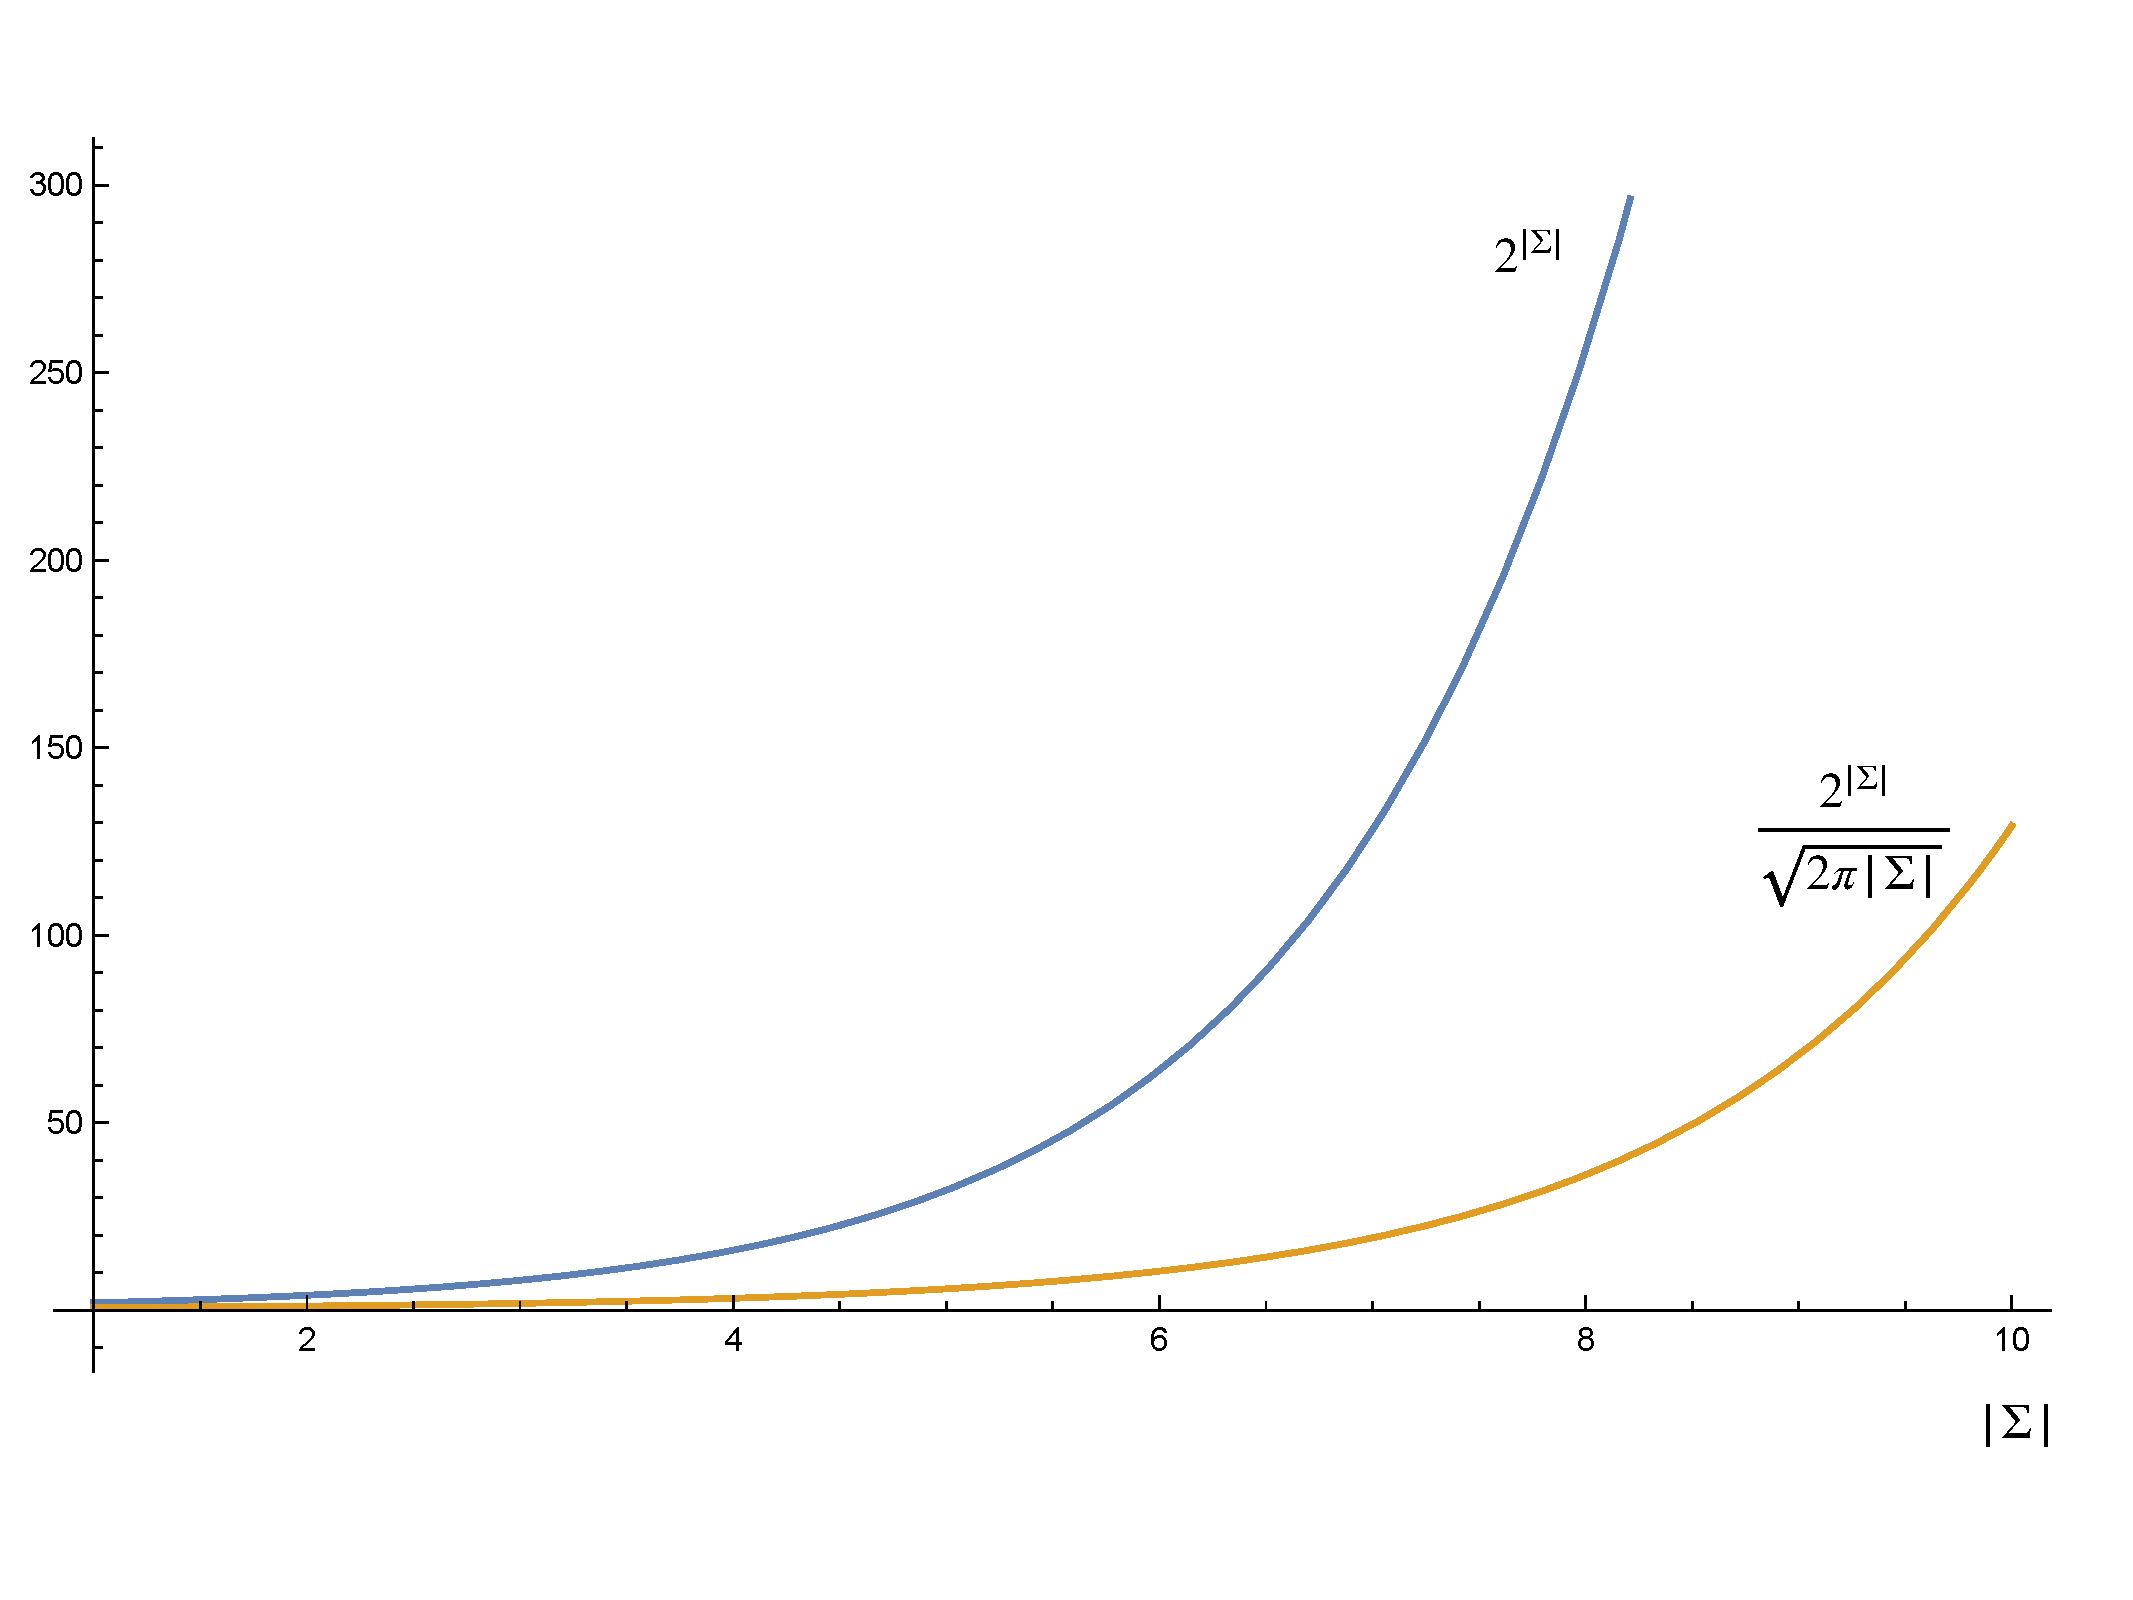
\includegraphics[width=.8\textwidth]{minhit-fig.pdf}
\end{center}
\vspace*{-10mm}
\caption{Function plot $2^{\card{\Sigma}}$ versus $\frac{2^\card{\Sigma}}{\sqrt{2\pi \card{\Sigma}}}$.}
 \label{fig:minhita}
 \end{figure}
% .......................................................................................

% -------------------------------------------------------------------------
\subsection{Upper Bounds of Test Executions for Checking Trace Refinement}

According to Theorem~\ref{th:tracetest}, a complete test suite checking trace
refinement just contains the adaptive test case $U_T(pq-1)$. As derived for
$U_F(j)$ above, the number of executions performed by $(Q\parallel[\Sigma]
U_T(pq-1))$ is bounded by $\card{\Sigma}^{pq-1}$.

% -------------------------------------------------------------------------
\subsection{Upper Bound $pq$ for the Maximal Length of Test Traces}

According to Theorem~\ref{th:failurestest}, the tests $U_F(j)$ need to be
executed for $j = 0,\dots,pq-1$ to guarantee completeness.
 This means that the SUT is verified with test
traces up to, and including, length $pq$: recall from the test specification,
branch (\ref{eq:ufa}), that $U_F(j)$ will accept all traces $s.e$ with
$s\in\trc(P), \#s = j, e\not\in\trc(P/s)$, so erroneous traces up to length
$j+1$ are detected.

It is interesting to investigate whether this maximal length is really
necessary, or whether one could elaborate alternative complete test
strategies where the SUT is tested with shorter traces only. Indeed, an
example  presented in~\cite[Exercise~5]{PeleskaHuangLectureNotesMBT} shows
that when testing for equivalence of deterministic FSMs, it is sufficient to
test the SUT with traces of significantly shorter length.

The following example, however, shows that the maximal length $pq$ is really
required when testing for refinement.
%\begin{example}\label{ex:pq}
%Consider the CSP reference process $P$ and an erroneous implementation $Q$
%specified as follows.
%
%\begin{center}
%\begin{minipage}{.4\textwidth}
%\begin{eqnarray*}
%P & = & a \then P_1 \intchoice b \then P_1 \intchoice c \then P_1
%\\
%P_1 & = & a \then P \extchoice b\then P
%\end{eqnarray*}
%\end{minipage}
%\hfill
%\begin{minipage}{.4\textwidth}
%\begin{eqnarray*}
%Q & = & a\then Q_1 \extchoice b\then Q_1
%\\
%Q_1 & = & a\then Q_2 \extchoice b\then Q_2
%\\
%Q_2 & = & a\then Q \intchoice b\then Q
%\end{eqnarray*}
%\end{minipage}
%\end{center}
%
%
%\medskip
%Obviously, $P$'s normalised transition graph has 2 nodes, while $Q$'s graph
%has 3. It is easy to see (and can be checked with FDR4) that $P\lessdet_T Q$,
%but $\neg(P\lessdet_F Q)$. Furthermore, it can also be shown using FDR4 that
%the ``test passed condition''
%\[
%(\epass\then\Stop) \lessdet_F (Q\parallel[\Sigma] U_F(j))\hide \Sigma
%\]
%holds for $U_F(0),\dots,U_F(4)$, but fails for $U_F(5)$. So, the
%non-conformance of $Q$ cannot be detected by any test trace of length less or
%equal to 5, but is revealed (as expected from Theorem~\ref{th:failurestest})
%by a trace of length 6, because the last event offered by the test $U_F(5)$
%is refused by $Q$. \xbox
%\end{example}

\begin{figure}[htbp]
\begin{center}
\begin{minipage}{.4\textwidth}
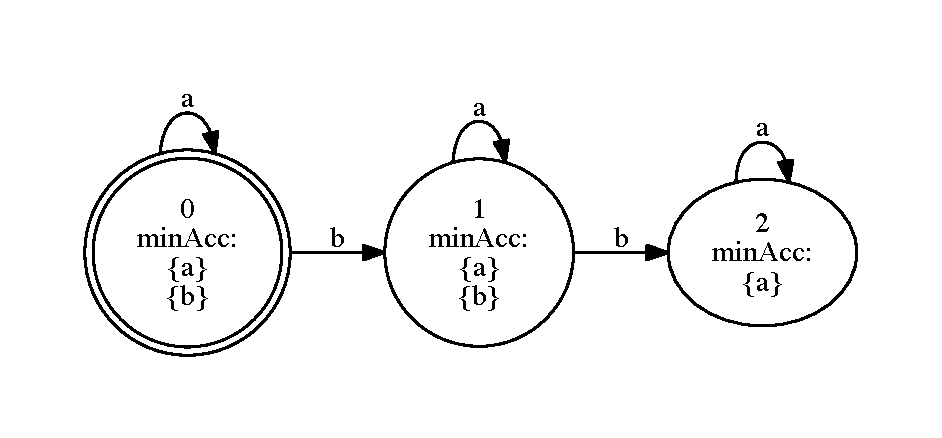
\includegraphics[width=1.2\textwidth]{theorem5p.pdf}
\end{minipage}
\hfill
\begin{minipage}{.55\textwidth}
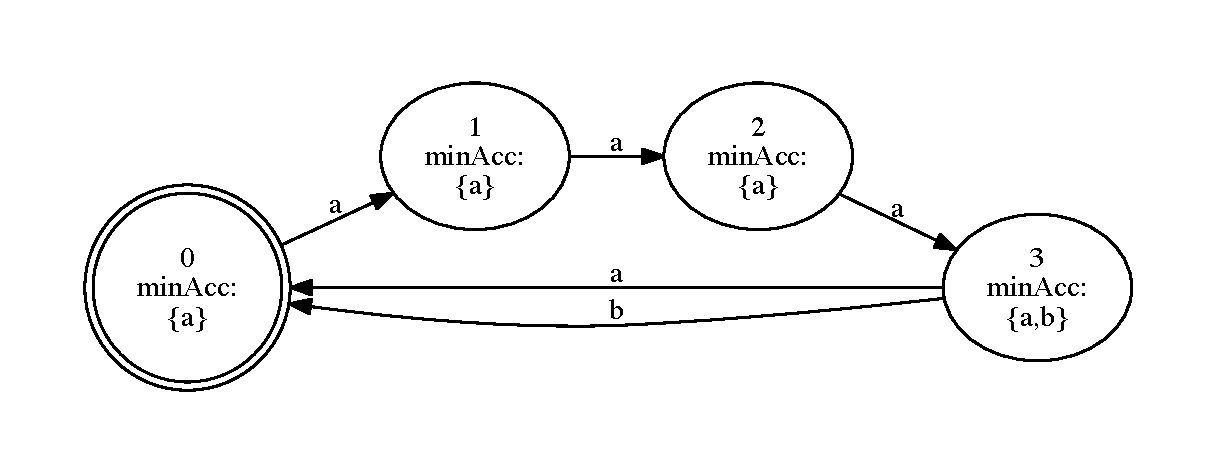
\includegraphics[width=1.2\textwidth]{theorem5q.pdf}
\end{minipage}
\caption{Transition graphs of $P$ (left) and $Q$ (right) from Example~\ref{ex:pq}
 for $p=3$ and $q=4$.}
\label{fig:examplepq}
\end{center}
\end{figure}

\begin{example}\label{ex:pq}
Consider the CSP reference process $P$ and an erroneous implementation $Q$
specified as follows.
%
\begin{eqnarray*}
P & = &  P(0)
\\
P(k) & = & (k < p-1) \& \big( (a \then P(k)) \intchoice ( b \then P(k+1))\big)
\\ & & \extchoice
\\ & & (k = p-1) \& (a \then P(k))
\\
Q & = & Q(0)
\\
Q(k) & = & (k < q-1) \& \big( a \then Q(k+1)    \big)
\\ & & \extchoice
\\ & & ( k = q-1)\& \big( a\then Q(0) \extchoice b\then Q(0)  \big)
\end{eqnarray*}
%
The normalised transition graphs of $P$ and $Q$ are depicted in
Fig.~\ref{fig:examplepq} for the case $p=3,\ q=4$. Using FDR4, it can be
shown for concrete values of $p$ and $q$ that the  ``test passed conditions''
\[
(\epass\then\Stop) \lessdet_F (Q\parallel[\Sigma] U_F(j))\hide \Sigma
\]
and
\[
(\epass\then\Stop) \lessdet_T (Q\parallel[\Sigma] U_T(j))\hide \Sigma
\]
hold for $j = 0,\dots,pq-2$. This means that none of the test cases $U_F(j)$
and $U_T(j)$ are capable of detecting failures and trace refinement
violations, if they only check traces up to length $pq-1$
(recall that this corresponds to $j\le pq-2$).

Process $Q$, however, neither conforms to $P$ in the failures refinement
relation, nor in the trace
refinement relation. This can only be seen when executing the test $U_F(pq-1)$ and
$U_T(pq-1)$, respectively. These tests fail, so this shows that $P\not\lessdet_F Q$ and
$P\not\lessdet_T Q$ according to Theorem~\ref{th:failurestest} and Theorem~\ref{th:tracetest}. Moreover, this shows that
the maximal trace
length $pq$ to be investigated in the tests cannot be further reduced without losing
the completeness property of the test suites.
\xbox
\end{example}
%
Generalising Example~\ref{ex:pq}, it can be shown that for any pair
$2\le p,q \in\mathbb{N}$,
there exist reference processes $P$ with $p$ states
and implementation processes $Q$ with $q$ states, such that
a violation of the trace refinement property
can only be detected with a trace of length $pq$. This is proven in the following
theorem. In the proof, we use the processes $P$ and $Q$ introduced in Example~\ref{ex:pq}.

% ----------------------------------------------------------------------------
\begin{theorem}\label{th:maxtracelen}
Let $2\le p,q \in\mathbb{N}$. Then there exists a reference process $P$ and an
implementation process $Q$ with the following properties.
\begin{enumerate}
\item $G(P)$ has $p$ states.
\item $G(Q)$ has $q$ states.
\item $P\not\lessdet_T Q$, and therefore, also $P\not\lessdet_F Q$.
\item $\forall s\in\trc(Q): \#s < pq\implies s\in\trc(P)$.
\item $Q\ conf\ P$.
\end{enumerate}
As a consequence, the upper bound $pq$ for the length of traces to be tested when checking for failures refinement or trace refinement
cannot be reduced without losing the test suite's completeness property.
\end{theorem}
% ----------------------------------------------------------------------------
\begin{proof}
Given $2\le p,q \in\mathbb{N}$, define reference process $P$ and implementation process $Q$ as in Example~\ref{ex:pq}. It is trivial to see that
$G(P)$ has $p$ nodes and $G(Q)$ has $q$ nodes, so statements 1 and 2 of the theorem hold.

Using regular expression notation, the traces of $P$ can be specified as
\[
\trc(P) = \prefs\big(  (a^*b)^{p-1}a^* \big),
\]
where $\prefs(M)$ denotes the set of all prefixes of traces in $M\subseteq\Sigma^*$,
including the traces of $M$ themselves.
The traces of $Q$ can be specified by
\[
\trc(Q) = \prefs\big( (a^{q-1}(a|b))^*  \big).
\]
It is easy to see that $\trc(Q)\not\subseteq\trc(P)$; for example, the trace
$(a^{q-1}b)^p$ is in $\trc(Q)\setminus\trc(P)$, because $P$-traces may contain at most $p-1$ $b$-events. This proves statement~3 of the theorem.

Let $s \in\trc(Q)$ be any trace of length $\#s = pq-1$. Then $s$ can be represented
by $s = (a^{q-1}(a|b))^{p-1}a^{q-1} \in \prefs\big( (a^{q-1}(a|b))^*  \big)$.
Then $s$ is also an element of $\trc(P)$, because $(a^{q-1}(a|b))^{p-1}a^{q-1}$
is also contained in $\prefs\big(  (a^*b)^{p-1}a^* \big)$: this is easy to see, since
$\prefs\big(  (a^*b)^{p-1}a^* \big)$ contains all finite sequences of $a$-events,
where at most $p-1$ events $b$ have been inserted. This proves statement 4 of the theorem.

To prove statement~5, we observe that the specification of $P$ implies (the
expression $(s\cnt b)$ denotes the number of $b$-events occurring in trace $s$)
\[
\minaccs(P/s) = \left\{
\begin{array}{ll}
\{ \{a\}, \{b\} \} & \text{for all $s\in\trc(P)$ with $(s\cnt b) <p-1$.}
\\
\{ \{a\} \} & \text{for all $s\in\trc(P)$ with $(s\cnt b) = p-1$.}
\end{array}
\right.
\]
and
\[
\minaccs(Q/s) = \left\{
\begin{array}{ll}
\{ \{a\}  \} & \text{for all $s\in\trc(Q)$ with $\#s \neq 0\mod(q-1)$.}
\\
\{ \{a,b\} \} & \text{for all $s\in\trc(P)$ with $\#s = 0\mod(q-1)$.}
\end{array}
\right.
\]
As a  consequence, the minimal acceptance set $A_P = \{a\}$ which is
contained in every $\minaccs(P/s)$ fulfils $A_P \subseteq A_Q$ for
any $A_Q\in\minaccs(Q/s)$, when $s\in\trc(P)\cap \trc(Q)$. Now Lemma~\ref{lemma:tgtrcref},
(\ref{eq:failrefb}) can be applied to conclude that $Q\ conf\ P$.
\xbox
\end{proof}
%
Since Theorem~\ref{th:maxtracelen} just states that a violation of trace
refinement may remain undetected if only traces shorter than $pq$ are checked
during tests, it can also be applied to our trace refinement tests.
Therefore, test suites $\{ U_T(j) \}$ with $j<pq-1$ are not complete. It is
discussed in Section~\ref{sec:conc} how the number of test traces to be
executed by complete test suites for failures or trace refinement can still
be reduced {\it without} reducing the maximal length.

% =================================================================================
